\documentclass[a4paper,11pt]{jsarticle}
\usepackage[utf8]{inputenc}
\usepackage[T1]{fontenc}
\usepackage{amsmath,amssymb,bm}
\usepackage{graphicx}
\usepackage{hyperref}

\title{Theory of magnetic properties in the spin-triplet superconducting state of Sr$_2$RuO$_4$}
\author{Takuji Nomura, Hiroaki Ikeda, Dai S. Hirashima}
\date{}

\begin{document}
\maketitle

\section*{アブスト}
我々は、Sr$_2$RuO$_4$の三重項対形成状態における磁化率を解析する。具体的には、キラル$p$波状態
$\bm{d}(\bm{k})=(k_x + i k_y)\hat{\bm{z}}$を仮定している。本論文は二つの独立した部分から構成されている。  
前半では、三バンドの斥力ハバードモデルを出発点とし、ランダム位相近似(RPA)を用いて、NMR緩和率
$(1/T_1)$を温度の関数として計算する。後半では、有効な三重項ペアリング相互作用を含む別のモデルを用い、長波長領域におけるスピンの集団励起(collective spin excitation)の可能性について議論する。  

いずれの解析においても、Sr$_2$RuO$_4$の現実的なマルチバンド電子構造を完全に考慮しており、電子相関効果からミクロ的に決定された超伝導ギャップを使用している。

\section{問題意識}
\begin{itemize}
  \item スピントリプレット超伝導体の最有力候補の一つに Sr$_2$RuO$_4$ がある。
  \item Sr$_2$RuO$_4$ における最有力な秩序変数は
    \[
      \bm{d}(\bm{k}) = (k_x + i k_y)\hat{\bm{z}}
    \]
    である。この応対でクーパー対のスピンは基底面内に揃い、基底面内ではキラル$p$波状態が実現される。トリプレット超伝導体では転移温度以下でもスピン回転自由度が完全には失われず、磁気的性質において異常な振る舞いが現れることがある。
  \item 本論文では、スピントリプレット対形成状態における磁気的性質を、現実的な多バンド電子構造と超伝導ギャップを用いて解析する。
\end{itemize}

\section{モデルと手法}
Ru 4$d$軌道に基づく3バンド模型を考える。
\begin{equation}
H_0 = \sum_{\bm{k}, \ell, s} \xi_\ell(\bm{k}) \, c^\dagger_{\ell \bm{k} s} c_{\ell \bm{k} s}
      + \sum_{\bm{k}, s} \lambda(\bm{k})
      \bigl(c^\dagger_{yz,\bm{k}s} c_{xz,\bm{k}s} + \mathrm{h.c.}\bigr).
\end{equation}
各軌道の分散は以下のようである。
\begin{align}
\xi_{xy}(\bm{k}) &= -2t_1(\cos k_x + \cos k_y) - 4t_2 \cos k_x \cos k_y - \mu_{xy},\\
\xi_{yz}(\bm{k}) &= -2t_3 \cos k_y - 2t_4 \cos k_x - \mu_{yz},\\
\xi_{xz}(\bm{k}) &= -2t_3 \cos k_x - 2t_4 \cos k_y - \mu_{xz},\\
\lambda(\bm{k})  &= -4t_5 \sin k_x \sin k_y.
\end{align}

相互作用は以下を仮定する。
\begin{equation}
H_{\mathrm{Coulomb}} = \frac{1}{2} \sum_{i} \sum_{z_1,z_2,z_3,z_4}
I_{z_1 z_2; z_3 z_4} \,
c^{\dagger}_{i z_1} c^{\dagger}_{i z_2} c_{i z_3} c_{i z_4},
\end{equation}
ここで $I_{z_1 z_2; z_3 z_4}$ はクーロン相互作用の行列要素であり、intra-orbitalの斥力$U$, inter-orbitalの斥力$U'$, Hund結合$J$, ペアホッピング$J'$ が含まれる。

スピン軌道相互作用は
\begin{equation}
H_{\mathrm{SO}} = \xi_{\mathrm{SO}}
\sum_{\bm{k}} \sum_{\ell,\ell',s,s'}
\bigl[\bm{l}\cdot\bm{s}\bigr]^{\ell s,\ell' s'}
c^\dagger_{\ell \bm{k} s} c_{\ell' \bm{k} s'}.
\end{equation}

グリーン関数と異常グリーン関数は
\begin{align}
G_{a s s'}(\bm{k}, i\omega_n) &= -\frac{i\omega_n + \xi_a(\bm{k})}{Z_a(\bm{k})} \,\delta_{s s'},\\
F_{a s s'}(\bm{k}, i\omega_n) &= \frac{\Delta_{a s s'}(\bm{k})}{Z_a(\bm{k})},\\
Z_a(\bm{k}) &= \omega_n^2 + \xi_a(\bm{k})^2 + \lvert \bm{d}_a(\bm{k}) \rvert^2.
\end{align}

ベアの感受率は
\begin{equation}
\chi^{(0)}_{z_1 z_2; z_3 z_4}(\bm{q})
= -T \sum_{\bm{k}}
\Bigl[
G_{z_4 z_1}(\bm{k})\,G_{z_2 z_3}(\bm{k} + \bm{q})
- F_{z_4 z_2}(\bm{k})\,F^\dagger_{z_1 z_3}(\bm{k} + \bm{q})
\Bigr].
\end{equation}

繰りこまれた磁化率は行列表記で
\begin{equation}
\hat{\chi}^{\mathrm{RPA}}(\bm{q})
= \bigl[\hat{1} - \hat{\chi}^{(0)}(\bm{q})\,\hat{G}^{\mathrm{RPA}}\bigr]^{-1}
  \hat{\chi}^{(0)}(\bm{q}),
\end{equation}
\begin{align}
[\hat{1}]_{z_1 z_2; z_3 z_4}
&= \delta_{z_1 z_3}\,\delta_{z_2 z_4},\\
[\hat{G}^{\mathrm{RPA}}]_{z_1 z_2; z_3 z_4}
&= I^{\mathrm{RPA}}_{z_1 z_3; z_2 z_4}
- I^{\mathrm{RPA}}_{z_1 z_3; z_4 z_2}.
\end{align}

物理量への投影は
\begin{equation}
\chi^{\mathrm{RPA}}_{mn}(\bm{q})
= \sum_{z_1,\dots,z_4}
[m_m]_{z_1 z_2}\,[m_n]_{z_3 z_4}\,
\chi^{\mathrm{RPA}}_{z_1 z_2; z_3 z_4}(\bm{q}).
\end{equation}

NMR緩和率は
\begin{equation}
\bigl(\tfrac{1}{T_1}\bigr)_{mn}
= T \sum_{\bm{q}}
\frac{\Im\,\chi^{\mathrm{RPA}}_{mn}(\bm{q},\omega + i0)}{\omega}
\biggr\rvert_{\omega \to 0},
\end{equation}
転移温度は $T_c \approx 0.019$ である。

\begin{figure}[htbp]
  \centering
  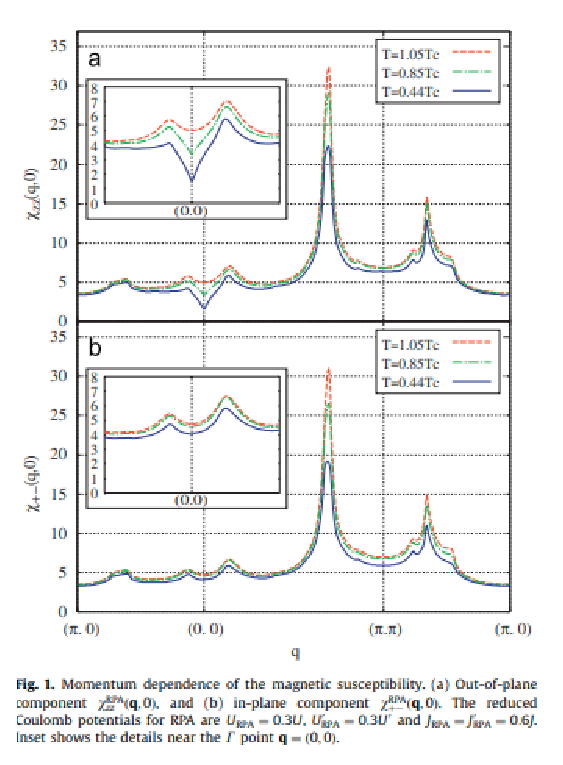
\includegraphics[width=\textwidth]{image-17.eps}
  \caption{Brillouin ゾーン中心付近での $\chi_{zz}$ の抑制。}
\end{figure}

\begin{figure}[htbp]
  \centering
  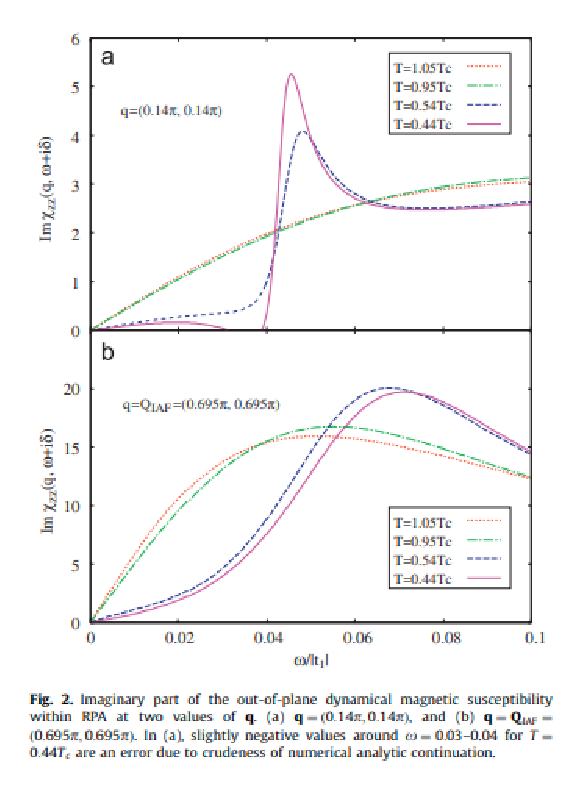
\includegraphics[width=\textwidth]{image-18.eps}
  \caption{$\chi_{zz}^{\mathrm{RPA}}$ の虚部(2 種類の $\bm{q}$ 点)。}
\end{figure}

\begin{figure}[htbp]
  \centering
  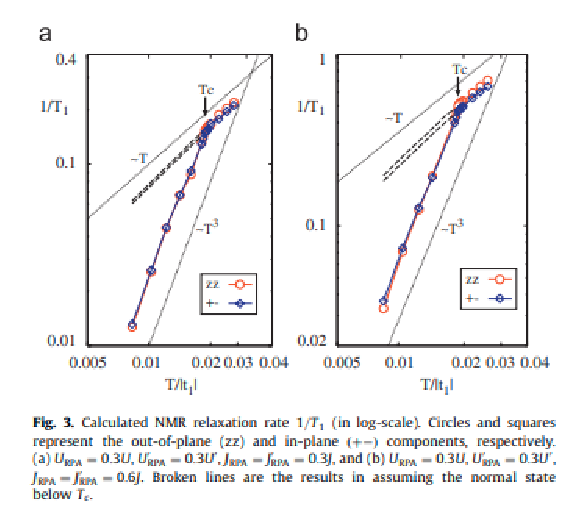
\includegraphics[width=\textwidth]{image-19.eps}
  \caption{NMR 緩和率の温度依存性。Hebel–Slichter ピークの不在と $T^3$ 依存性。}
\end{figure}

\section*{問題点}
\begin{itemize}
  \item 実験で観測されている NMR 緩和率の異方性を本研究の結果は定量的に再現できていない。
  \item 反強磁性波数での RPA 磁化率異方性も中性子散乱実験の値を説明するには小さすぎる。
\end{itemize}

集団スピン励起について、有効な三重項ペアリング相互作用
\begin{align}
H_{\mathrm{eff}} &= -\tfrac{1}{2}\sum_{n=x,y,z} g_n
  \sum_{a,a'} \sum_{\bm{k},\bm{k}',\bm{q}}
  \sum_{s_1,\dots,s_4} \sum_{l=x,y}
  f_a^l(\bm{k}) f_{a'}^l(\bm{k}')
  \nonumber\\
&\quad\times (\sigma_n\sigma_y)_{s_1 s_2} (\sigma_y\sigma_n)_{s_3 s_4}
  \,c^\dagger_{a,\bm{k}+\bm{q}/2,s_1}
  c^\dagger_{a,-\bm{k}+\bm{q}/2,s_2}
  \nonumber\\
&\quad\quad\times c_{a',-\bm{k}'+\bm{q}/2,s_3}
  c_{a',\bm{k}'+\bm{q}/2,s_4}
\end{align}
を導入する。平均場近似では $g_z > g_x = g_y$ ならば秩序パラメータ $\bm{d}(\bm{k})\parallel\hat{\bm{z}}$ が実現し、対応するゴールドストンモードがスピン波モードとして出現する。ペアリング相互作用が異方的である場合、このスピン励起モードはギャップを持つ。

\begin{figure}[htbp]
  \centering
  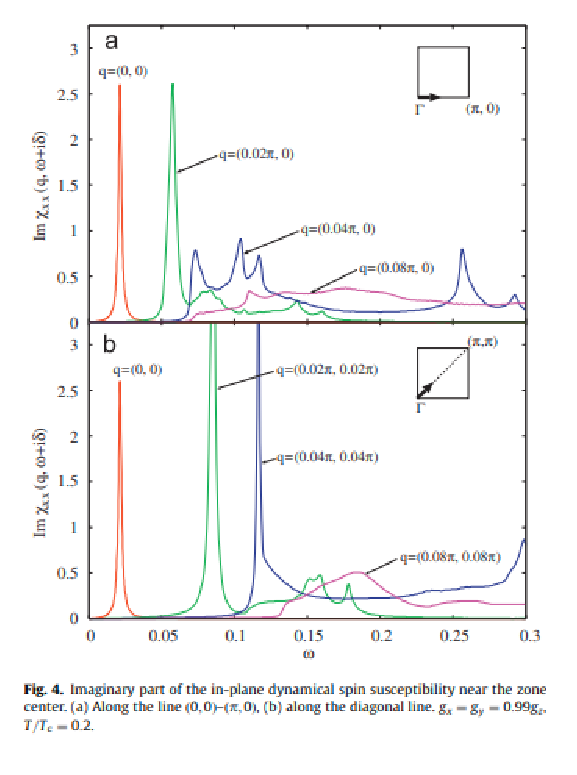
\includegraphics[width=\textwidth]{image-20.eps}
  \caption{多バンド計算における面内動的スピン感受率のポールとして現れる集団スピン励起モード。}
\end{figure}

\section*{感想・メモ}
\begin{itemize}
  \item 集団励起モードの計算では、超伝導転移温度を $T_c = 0.05$ とやや高めに設定しているらしい。
\end{itemize}

\end{document}
